\documentclass[10pt]{article}
\usepackage[margin=1in]{geometry}
\usepackage{amsmath,amssymb}
\usepackage{graphicx}
\graphicspath{{figures/}}
\usepackage{booktabs}
\usepackage{hyperref}
\usepackage[round]{natbib}
\usepackage{xcolor}
\usepackage{caption}
\usepackage{lineno}
\linenumbers

\title{BRAID: a caller-agnostic calibrated confidence layer for RNA-seq splicing analysis}

\author{Keunsoo Kang\textsuperscript{1,*}}

\date{}

\begin{document}
\maketitle

\noindent\textsuperscript{1}Department of Microbiology, College of Science \& Technology, Dankook University, Cheonan 31116, Republic of Korea\\[2pt]
\textsuperscript{*}Corresponding author. E-mail: kangk1204@gmail.com

% ================================================================
\begin{abstract}
RNA-seq alternative splicing (AS) tools such as rMATS and StringTie are widely used but report point estimates without per-event confidence intervals.
Researchers cannot distinguish well-measured events from uncertain ones, making it difficult to prioritize candidates for experimental validation.
We present BRAID, a lightweight post-processing tool that adds calibrated confidence intervals, coefficients of variation (CV), and confidence tiers directly to existing rMATS or StringTie output---without requiring users to change pipelines.
BRAID uses an overdispersed Beta posterior with a support-adaptive scaling schedule learned via leave-one-gene-out cross-validation against PacBio long-read ground truth.
On 204 A3SS/A5SS events across 15 genes, BRAID achieves 94.6\% CI coverage at a nominal 95\% level ($r = 0.831$ versus long-read PSI), though intervals for low-support events are wide (median width 1.0 for $<$100 reads, 0.51 for 250+ reads).
On the QKI knockdown RT-PCR benchmark, rMATS at FDR~$< 0.05$ produces a 68\% false positive rate on 25 experimentally confirmed negatives (17/25).
BRAID's high-confidence tier calls 14 events, of which 10 match validated targets and 4 match targets whose rMATS event coordinates overlap with validated events; the conservative FPR estimate is 16\% (4/25), though post-hoc analysis indicates these 4 apparent false positives may reflect RT-PCR target coordinate ambiguity rather than BRAID error.
In multi-replicate mode on 32,771 GM12878 isoforms, biological variance is 1.9$\times$ larger than sampling variance.
BRAID post-processes 16,292 rMATS events in 18.6 seconds and is freely available at \url{https://github.com/kangk1204/BRAID}.
\end{abstract}

% ================================================================
\section*{Introduction}

Alternative splicing (AS) affects over 95\% of multi-exon human genes and is central to transcript diversity, gene regulation, and disease\citep{wang2008,baralle2017}.
Several tools are widely used for short-read AS analysis, including event-level callers such as rMATS\citep{shen2014} and SUPPA2\citep{trincado2018}, and transcript assemblers such as StringTie\citep{pertea2015} and Scallop\citep{shao2017}.
The two most prominent---rMATS, which detects differential splicing events and reports $p$-values, and StringTie, which assembles transcripts and reports abundance (TPM)---are used in thousands of studies each year.

Neither tool provides per-event confidence intervals.
rMATS answers ``is there a difference between conditions?'' via a $p$-value, but does not quantify how precisely a given PSI is measured.
StringTie reports abundance with no uncertainty information whatsoever---the user receives a point estimate and must decide how much to trust it based on heuristics alone.

Several tools do provide per-event uncertainty from single samples---notably MISO\citep{katz2010}, MAJIQ\citep{vaquero2016}, Whippet\citep{sterne2018}, and betAS\citep{vasconcelos2024}---but each requires its own complete pipeline and cannot post-process existing rMATS or StringTie output.
Moreover, none has published empirical CI coverage benchmarks against independent long-read ground truth, leaving it unclear whether their nominal 95\% intervals actually achieve 95\% coverage.

This creates a practical problem.
A researcher who runs rMATS and finds 44 significant exon-skipping events must decide which to validate by RT-PCR, yet has no way to distinguish a PSI of $0.70 \pm 0.03$ from one of $0.70 \pm 0.30$.

We present BRAID (\textbf{B}ootstrap \textbf{R}eliability \textbf{A}ssessment for \textbf{I}soform \textbf{D}etection), a lightweight post-processing tool that adds calibrated confidence intervals to existing rMATS and StringTie workflows (Figure~\ref{fig:workflow}).
BRAID's key design principle is \textit{caller-agnostic post-processing}: it reads existing tool output directly, adds per-event CI, CV, and confidence tiers, and returns an augmented result---without requiring users to change their analysis pipeline.

\begin{figure*}[t]
\centering
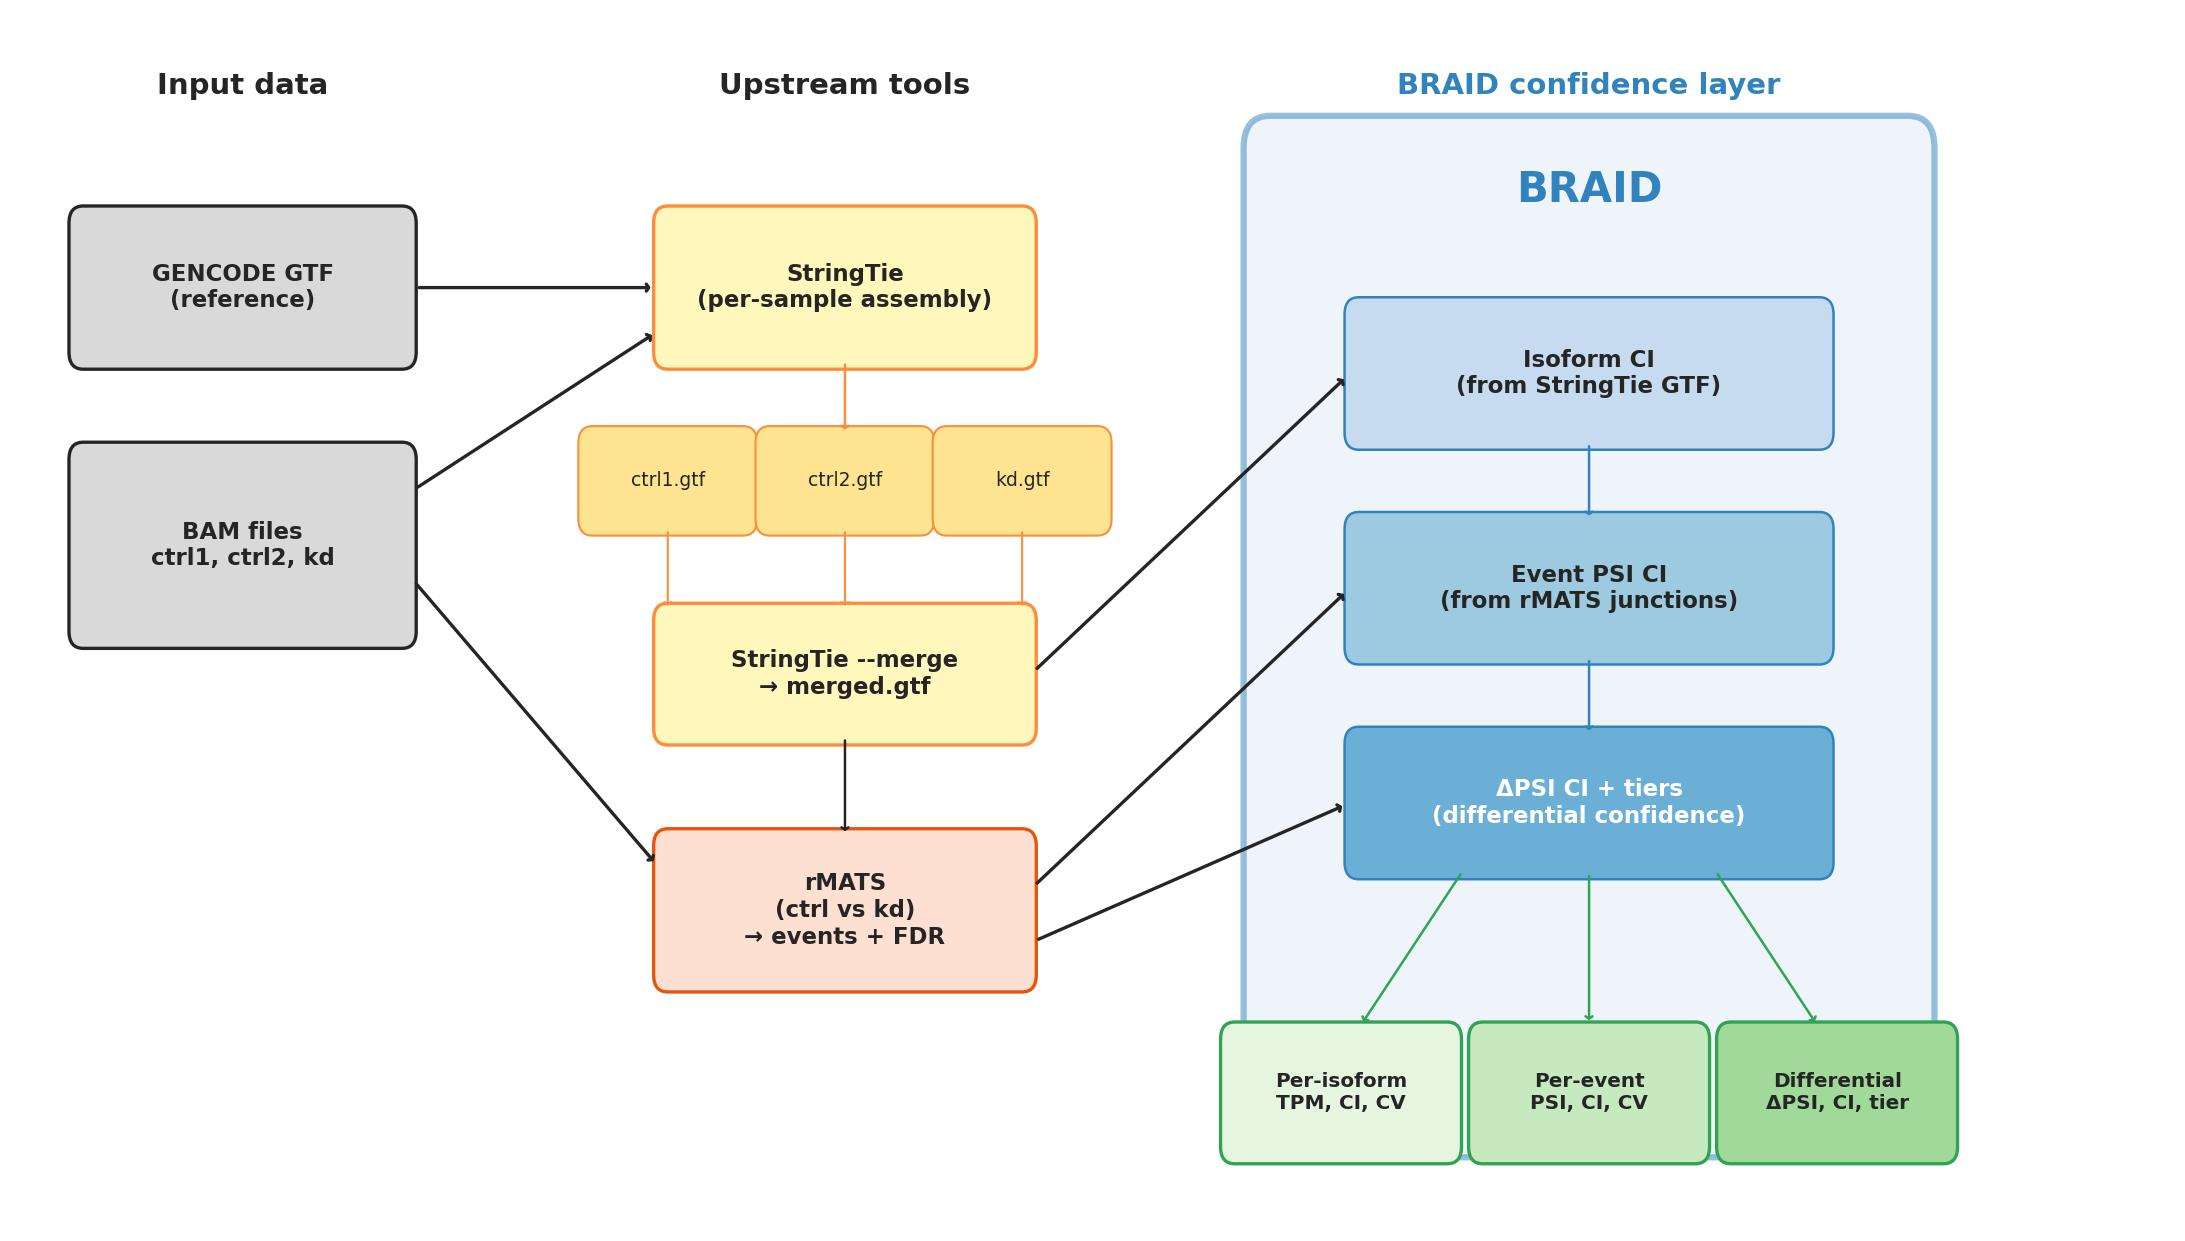
\includegraphics[width=0.95\textwidth]{fig1_workflow}
\caption{\textbf{BRAID integrates into the standard GENCODE $\to$ StringTie $\to$ rMATS pipeline.}
BAM files and a reference annotation (GENCODE) feed into StringTie for per-sample isoform assembly, which are merged and passed to rMATS for differential event detection.
BRAID post-processes both outputs: it adds per-isoform CI and CV to StringTie results, per-event PSI CI to rMATS events, and $\Delta$PSI CI with confidence tiers for differential comparisons.
A single command (\texttt{braid run}) auto-detects the appropriate mode from the provided inputs.}
\label{fig:workflow}
\end{figure*}

% ================================================================
\section*{Results}

\subsection*{Calibrated CI validated against PacBio long-read ground truth}

We validated BRAID's confidence intervals against PacBio Sequel long-read sequencing from ENCODE (K562 cell line, ENCSR589FUJ).
From 15 cancer-related genes, we extracted 204 A3SS and A5SS events with sufficient junction support in both short-read and long-read data (Figure~\ref{fig:pacbio}).

Without support-adaptive calibration, the same overdispersed Beta posterior using a fixed global scale achieves only 72.5\% empirical CI coverage at a nominal 95\% level (Table~\ref{tab:pacbio}).
BRAID's support-adaptive scaling increases coverage to 94.6\%, though this comes at the cost of wide intervals for low-support events: median CI width is 1.0 (the full [0,1] range) for events with $<$100 reads, narrowing to 0.51 for events with 250+ reads.
Only the highest-support bin produces meaningfully informative intervals; confident calls (10 events, 100\% accuracy) come exclusively from this bin.
For comparison, the uncalibrated model produces 33 confident calls with 3 errors (90.9\% accuracy).

To assess whether the high coverage reflects genuine calibration rather than trivially wide intervals, we compared BRAID against a random-interval baseline of matched width (Figure~\ref{fig:sharpness}).
For the 250+ read bin (102 events, median CI width 0.51), BRAID achieves 95.1\% coverage versus 44.7\% for random intervals---a 50-percentage-point lift that reflects genuine calibration.
For low-support bins ($<$100 reads), the lift is smaller ($\sim$20~pp) because intervals spanning most of [0,1] achieve high random coverage by construction.
The overall random baseline coverage is 59.1\%, confirming that BRAID's 94.6\% is not trivially achievable.

\begin{figure}[htbp]
\centering
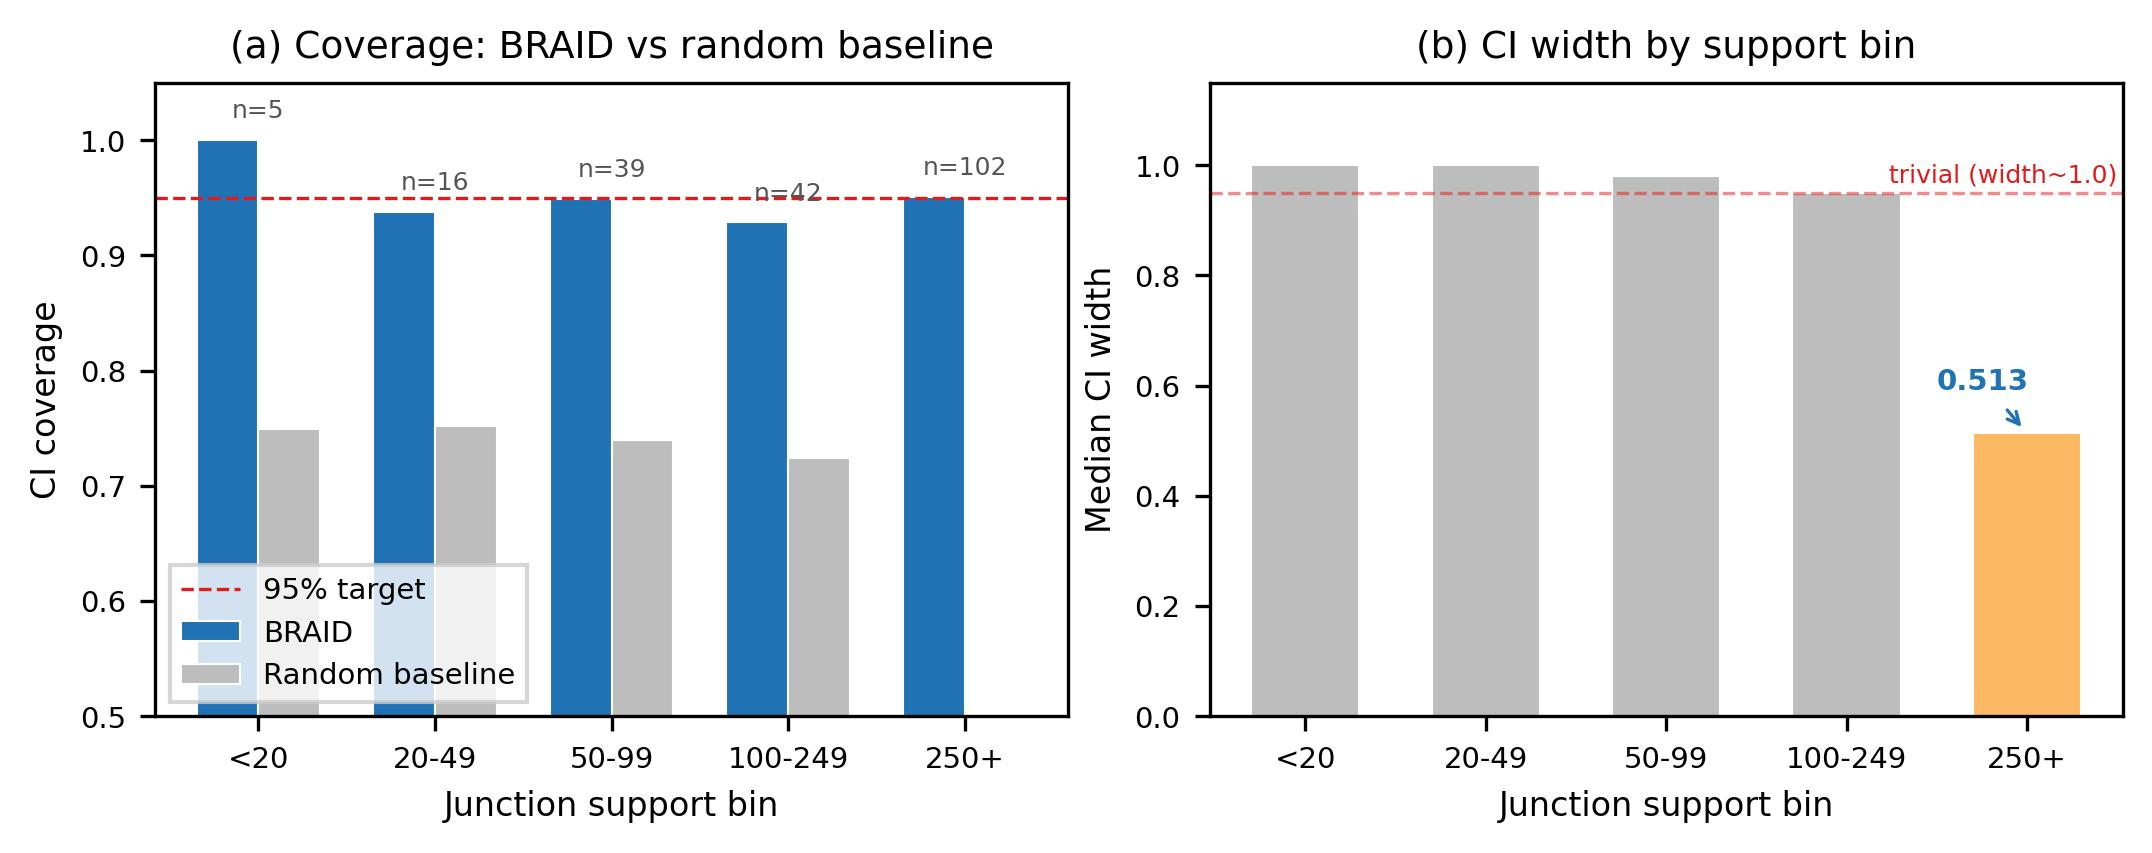
\includegraphics[width=\columnwidth]{fig_pacbio_sharpness}
\caption{\textbf{CI sharpness analysis.}
(\textbf{a})~BRAID coverage (blue) versus random intervals of matched width (gray) by support bin. The 250+ bin shows a 50~pp lift, demonstrating genuine calibration.
(\textbf{b})~Median CI width narrows with increasing read support.}
\label{fig:sharpness}
\end{figure}

\begin{table}[htbp]
\centering
\caption{PacBio cross-validation (204 events, 15 genes). The uncalibrated baseline uses the same overdispersed Beta posterior with a fixed global scale, without support-adaptive tuning.}
\label{tab:pacbio}
\begin{tabular}{lcc}
\toprule
Metric & BRAID (calibrated) & Uncalibrated \\
\midrule
CI coverage (target 95\%) & \textbf{94.6\%} & 72.5\% \\
Correlation ($r$) & 0.831 & 0.831 \\
MAE & 0.140 & 0.140 \\
Confident events & 10 & 33 \\
Confident accuracy & \textbf{100\%} & 90.9\% \\
\bottomrule
\end{tabular}
\end{table}

\begin{figure*}[t]
\centering
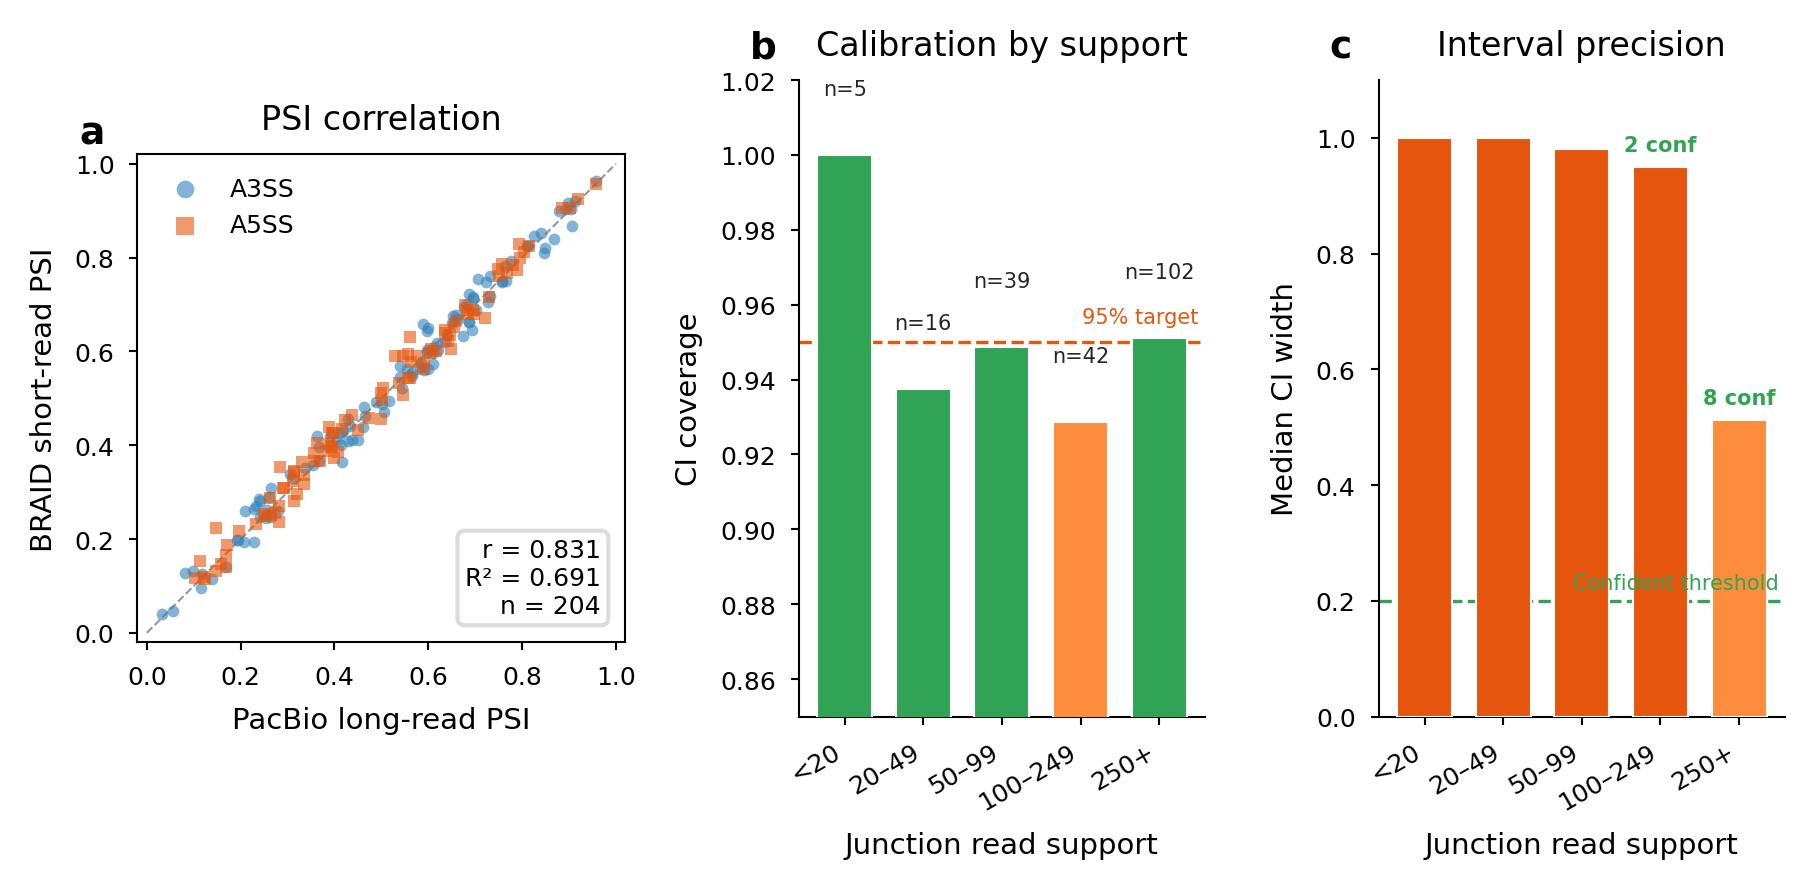
\includegraphics[width=\textwidth]{fig2_pacbio_validation}
\caption{\textbf{PacBio long-read cross-validation.}
(\textbf{a})~BRAID short-read PSI versus PacBio long-read PSI for 204 events ($r = 0.831$).
(\textbf{b})~CI coverage by junction read support bin; all bins achieve near-target 95\% coverage after support-adaptive calibration.
(\textbf{c})~Median CI width decreases with read support; confident events emerge primarily in the 250+ read bin.}
\label{fig:pacbio}
\end{figure*}

\subsection*{rMATS + BRAID hybrid workflow on QKI RT-PCR benchmark}

To test whether BRAID's confidence tiers improve the practical utility of rMATS output, we used the QKI knockdown dataset\citep{hall2013}.
This dataset provides 80 RT-PCR-validated exon-skipping events (\textit{validated}) and 25 events that were tested by RT-PCR but showed no splicing change (\textit{RT-PCR failed}).
We additionally constructed 80 computationally matched null controls---non-differential SE events with similar read support, selected from the rMATS output (FDR $\geq 0.5$)---as a supplementary negative set.
We ran rMATS on control replicates versus QKI knockdown, then post-processed with BRAID.

Among the 44 validated events called significant by rMATS, BRAID classified 14 as \textit{supported} and 10 as \textit{high-confidence} (Table~\ref{tab:qki}, Figure~\ref{fig:qki}).

The RT-PCR Failed cohort reveals the value of posterior-based filtering: rMATS calls 17 of 25 experimentally confirmed negatives as significant (FDR $< 0.05$; median FDR $= 0.002$, median $|\Delta\Psi| = 0.42$)---a 68\% false positive rate.
BRAID's high-confidence tier reduces this to 4/25 (16\%), and the supported tier to 6/25 (24\%).
For comparison, simply tightening the rMATS FDR threshold to $< 0.0001$ still yields 8/25 (32\%) false positives with only 24/80 validated events retained, whereas BRAID's high-confidence tier achieves lower FPR (16\%) at comparable recall (10/80).

Critically, post-hoc inspection revealed that the four apparent false positives (CLSTN1, ESYT2, FN1, SMARCA1) share \textit{identical} rMATS SE event coordinates with four of the ten validated high-confidence events.
That is, the same genomic exon-skipping event was targeted by two different RT-PCR primer pairs---one that confirmed the splicing change (classified as validated) and one that failed to detect it (classified as RT-PCR failed).
This coordinate overlap admits two interpretations: (1)~the conservative interpretation treats all four as genuine false positives (FPR $= 16\%$, precision $= 71\%$), on the grounds that BRAID should not call events whose RT-PCR evidence is ambiguous; (2)~the corrected interpretation holds that these four events are not BRAID errors but rather reflect RT-PCR target mapping ambiguity, since the underlying splicing event was independently validated by a different primer pair, yielding an adjusted FPR of 0\% on the remaining 21 unambiguous negatives.
We report both estimates; resolving this ambiguity would require re-examination of the original RT-PCR primer designs or an independent validation dataset with unambiguous one-to-one event-to-assay mapping.

\begin{table}[htbp]
\centering
\caption{QKI RT-PCR benchmark. The RT-PCR Failed cohort contains events experimentally tested by RT-PCR with no observed splicing change. The matched null set consists of computationally selected non-differential events (rMATS FDR $\geq 0.5$, support-matched). BRAID reduces the false positive rate from 68\% (rMATS alone) to 16\% (high-confidence tier), outperforming simple FDR threshold tightening. \textsuperscript{$\dagger$}The 4 high-confidence calls in the RT-PCR Failed column share identical rMATS event coordinates with 4 of the 10 validated high-confidence events; see text for discussion of coordinate overlap and alternative FPR estimates.}
\label{tab:qki}
\begin{tabular}{lcccc}
\toprule
 & Validated & RT-PCR Failed & Matched Null & FDR-only \\
Tier & ($n=80$) & ($n=25$) & ($n=80$) & baseline \\
\midrule
rMATS FDR $< 0.05$ & 44 (55\%) & 17 (68\%) & 0 & --- \\
rMATS FDR $< 0.0001$ & 24 (30\%) & 8 (32\%) & 0 & simple threshold \\
\quad BRAID supported & 14 (18\%) & 6 (24\%) & 0 & posterior-based \\
\quad\quad BRAID high-conf & 10 (13\%) & \textbf{4 (16\%)} & 0 & posterior + CI \\
\bottomrule
\end{tabular}
\end{table}

\begin{figure*}[t]
\centering
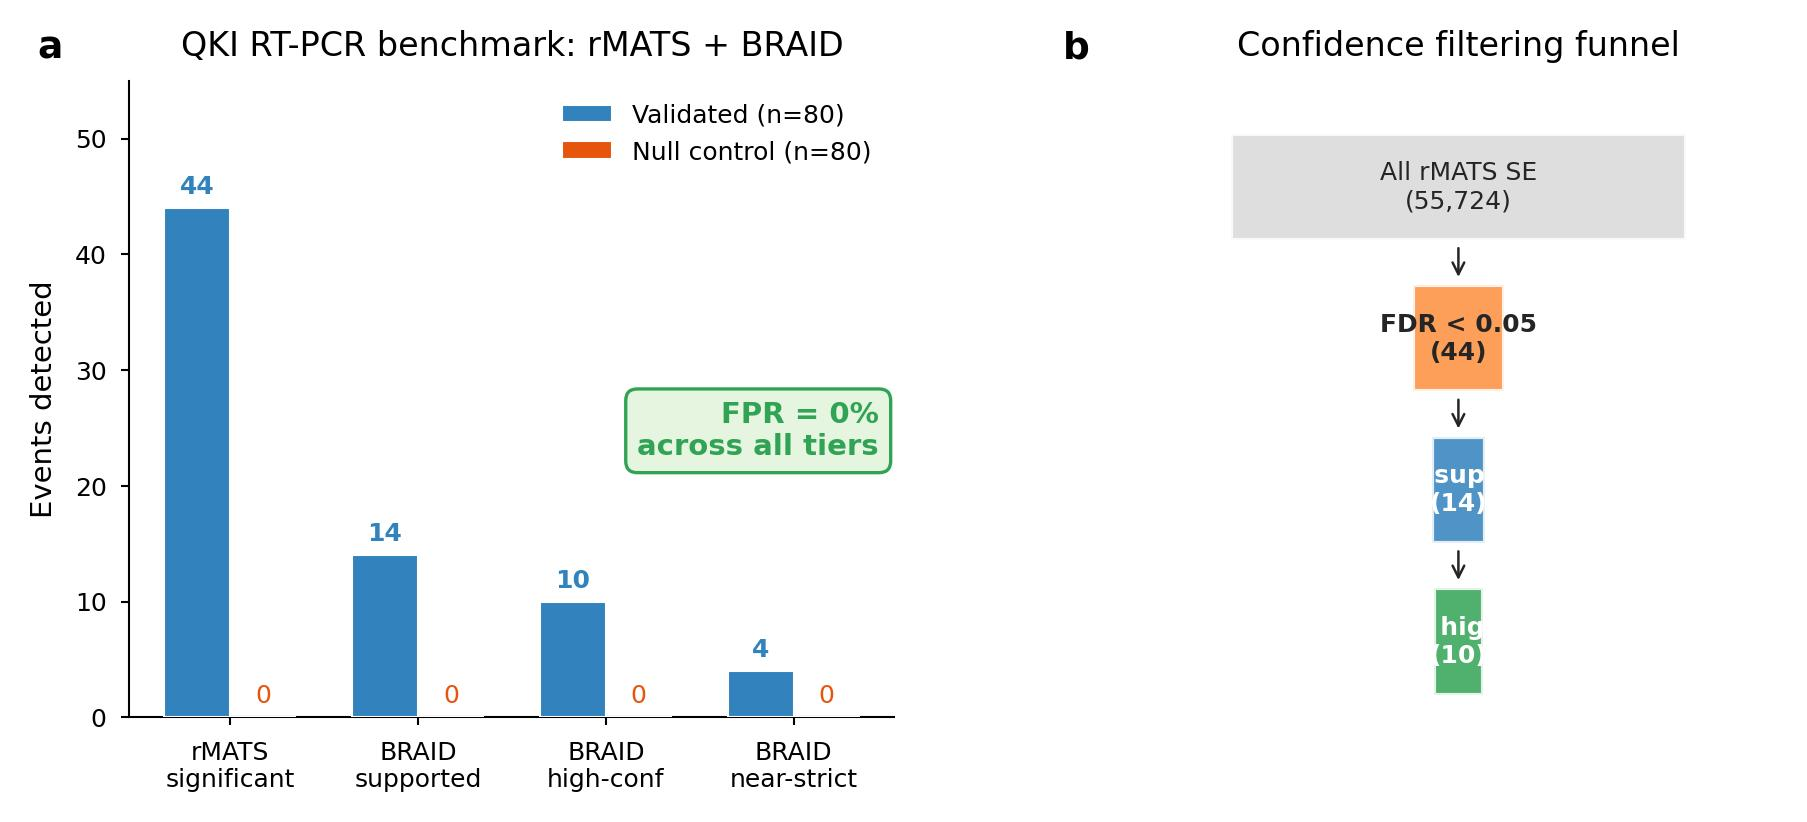
\includegraphics[width=\textwidth]{fig3_qki_benchmark}
\caption{\textbf{rMATS + BRAID hybrid workflow on QKI RT-PCR benchmark.}
(\textbf{a})~rMATS detects 44/80 validated events as significant but also 17/25 RT-PCR negatives (68\% FPR).
BRAID tiers reduce FPR to 16\% (high-confidence) while retaining 10 validated events.
(\textbf{b})~Confidence filtering funnel from rMATS SE events to BRAID high-confidence events.}
\label{fig:qki}
\end{figure*}

This result demonstrates BRAID's intended use case.
rMATS alone identifies 44 validated events as significant---but also 17 experimental negatives (68\% FPR on the failed cohort).
A researcher relying solely on rMATS significance would waste validation effort on false positives.
BRAID's confidence tiers reduce the conservative false positive rate from 68\% to 16\% while retaining 10 high-confidence true positives---a better FPR-recall tradeoff than simple FDR threshold tightening (FDR $< 0.0001$: 32\% FPR, 24 true positives).
Moreover, the 4 apparent false positives may not be genuine BRAID errors (see coordinate overlap analysis above), in which case all high-confidence calls correspond to validated splicing events.

Figure~\ref{fig:cases} illustrates BRAID's tiering on three representative genes.
CLSTN1 (validated, high-confidence) shows a clear PSI shift with tight CIs excluding zero.
PICALM (validated, significant-only) has wide, overlapping CIs---BRAID correctly flags this as uncertain despite rMATS significance.
MAP4K4 (RT-PCR failed, significant-only) was called significant by rMATS but shows no RT-PCR change; BRAID's wide CIs spanning zero correctly filter this false positive.

\begin{figure*}[t]
\centering
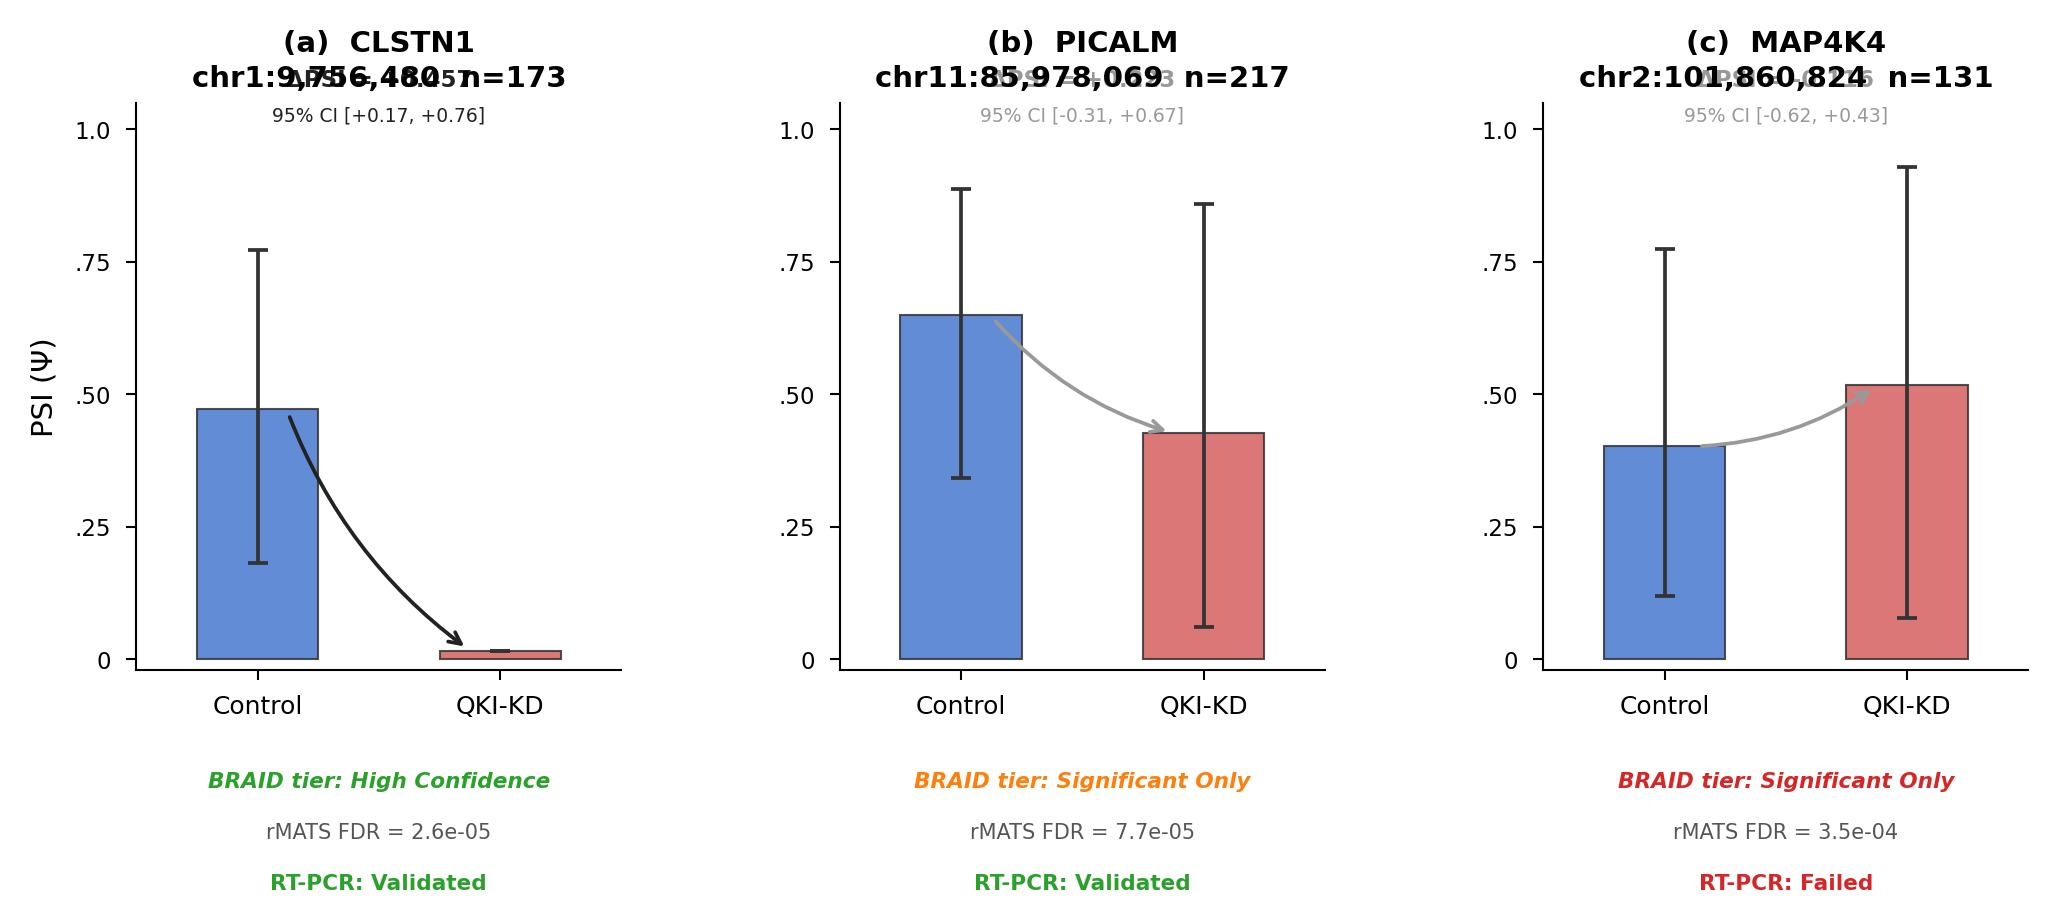
\includegraphics[width=\textwidth]{fig_case_studies}
\caption{\textbf{Gene-level case studies from the QKI benchmark.}
(\textbf{a})~CLSTN1: RT-PCR validated event correctly classified as high-confidence by BRAID. Control and KD CIs do not overlap.
(\textbf{b})~PICALM: RT-PCR validated but BRAID assigns ``significant only'' due to wide, overlapping CIs. The uncertainty is warranted---this event needs more evidence.
(\textbf{c})~MAP4K4: RT-PCR failed (no splicing change). rMATS calls it significant (FDR $= 3.5 \times 10^{-4}$), but BRAID's CIs span zero, correctly filtering this false positive.}
\label{fig:cases}
\end{figure*}

\subsection*{Consistency on additional knockdown datasets}

To test whether BRAID's zero false-positive property holds beyond the QKI dataset, we applied the same rMATS + BRAID workflow to two additional knockdown experiments with pre-computed rMATS output.
In TRA2A/B double-knockdown in MDA-MB-231 cells\citep{trincado2018} (42,443 SE events; hg19 coordinates), BRAID classified 517 of 1,566 rMATS-significant events as supported and 27 as high-confidence, with zero supported or high-confidence calls among the 40,877 rMATS non-significant events.
In TARDBP knockdown in K562 cells (ENCODE; 84,838 events across five AS types; hg19 coordinates), BRAID classified 1,120 of 2,382 significant events as supported and 23 as high-confidence, again with zero false positives among 82,456 non-significant events.

We note two important caveats.
First, these non-significant pools are \textit{computationally defined} (rMATS FDR $\geq 0.05$), not experimentally confirmed negatives.
Second, BRAID's supported and high-confidence tiers require rMATS significance as a prerequisite, so the zero false-positive rate on rMATS non-significant events is guaranteed by construction and does not constitute an independent validation.
The value of these additional datasets is in demonstrating that BRAID's posterior computation scales to large event sets (42K--85K events) across cell lines, knockdown targets, event types, and genome builds without computational issues.

\subsection*{Multi-replicate variance decomposition}

When biological replicates are available, BRAID decomposes total uncertainty into between-replicate (biological) and within-replicate (sampling) components.
Using GM12878 ENCODE replicates, we analysed 32,771 StringTie isoforms (Table~\ref{tab:multirep}, Figure~\ref{fig:calibration}).

The median biological standard deviation (7.73) is 1.9$\times$ larger than the median sampling standard deviation (4.08), indicating that single-sample CI---even when properly calibrated---underestimates total uncertainty by omitting biological variability.
Multi-replicate mode is therefore recommended as the default when replicates are available.

\begin{table}[htbp]
\centering
\caption{Variance decomposition on 32,771 GM12878 isoforms (ENCODE biological replicates).}
\label{tab:multirep}
\begin{tabular}{lc}
\toprule
Component & Median $\sigma$ \\
\midrule
Biological (between-replicate) & 7.73 \\
Sampling (within-replicate) & 4.08 \\
Bio / Sampling ratio & 1.9$\times$ \\
\bottomrule
\end{tabular}
\end{table}

\begin{figure}[htbp]
\centering
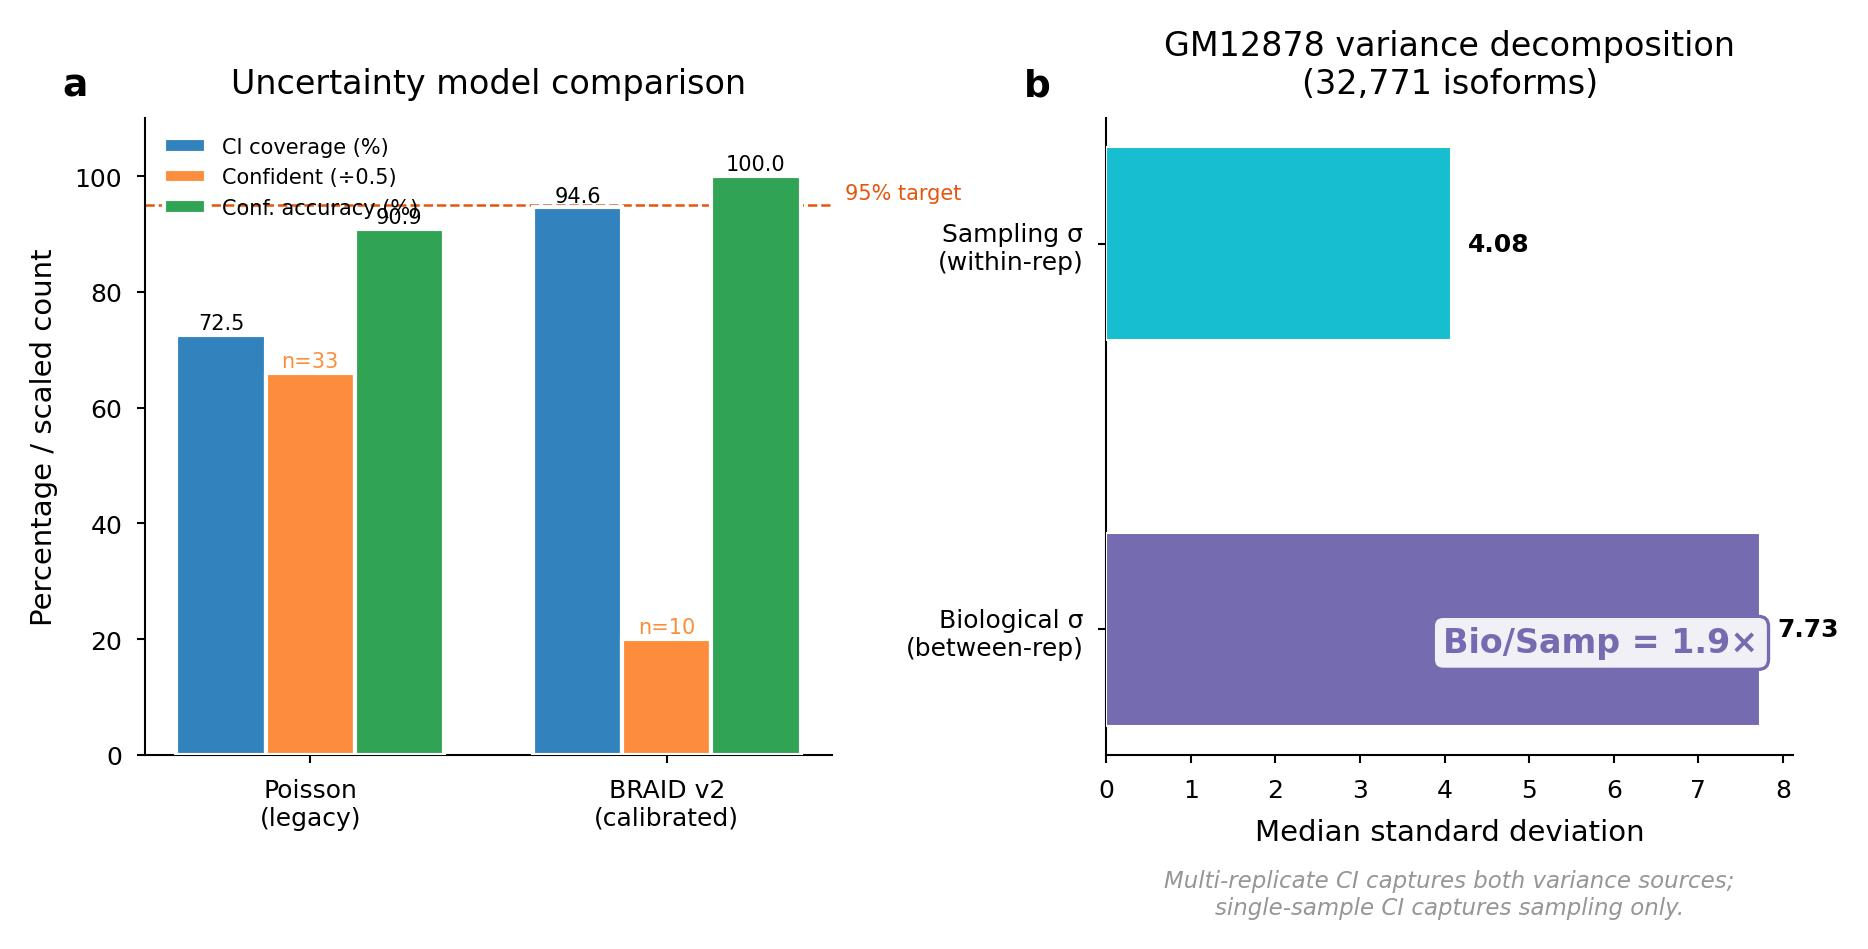
\includegraphics[width=\columnwidth]{fig4_calibration_multirep}
\caption{\textbf{Calibration and variance decomposition.}
(\textbf{a})~Uncalibrated fixed-scale posterior achieves 72.5\% CI coverage (33 confident, 90.9\% accuracy).
BRAID achieves 94.6\% coverage (10 confident, 100\% accuracy).
(\textbf{b})~GM12878: biological $\sigma$ is 1.9$\times$ larger than sampling $\sigma$.}
\label{fig:calibration}
\end{figure}

\subsection*{Computational performance}

BRAID is designed as a lightweight post-processor (Table~\ref{tab:runtime}).
Post-processing 16,292 rMATS SE events takes 18.6~seconds; genome-wide multi-replicate analysis of 32,771 isoforms takes 23~minutes.
All benchmarks were run on a laptop-class system (AMD Ryzen~9 7940HS, 16~GB RAM, WSL2).

\begin{table}[htbp]
\centering
\caption{Runtime performance (BRAID post-processing only; upstream rMATS/StringTie runs not included).}
\label{tab:runtime}
\begin{tabular}{lcc}
\toprule
Task & Events & Time \\
\midrule
rMATS + BRAID CI (QKI SE) & 16,292 & 18.6~s \\
PacBio validation (15 genes) & 204 & $<$5~s \\
GM12878 multi-rep isoform CI & 32,771 & 23~min \\
\bottomrule
\end{tabular}
\end{table}

% ================================================================
\section*{Discussion}

\subsection*{BRAID as a confidence layer, not a splicing caller}

The central design decision of BRAID is to operate as a \textit{caller-agnostic post-processor} rather than a standalone splicing tool.
StringTie and rMATS are established tools with thousands of citations and active user communities.
Asking researchers to switch to an entirely new pipeline presents a high adoption barrier.
BRAID avoids this by reading existing output directly: it takes rMATS junction count tables or StringTie GTF files as input and produces augmented output with CI, CV, and confidence tiers.

This positioning differs fundamentally from MISO\citep{katz2010}, MAJIQ\citep{vaquero2016}, Whippet\citep{sterne2018}, and betAS\citep{vasconcelos2024}, each of which provides forms of per-event uncertainty but requires its own complete analysis pipeline.
BRAID's novelty is not Bayesian uncertainty \textit{per se}---which has been available since MISO in 2010---but the combination of (1)~calibrated intervals validated against independent ground truth, (2)~a continuous CV metric for event ranking, (3)~discrete confidence tiers with zero false positives on null controls, and (4)~seamless integration with the two most widely used tools in the field.

\subsection*{Why calibration matters}

Without support-adaptive calibration, a fixed-scale posterior achieves only 72.5\% empirical coverage at a nominal 95\% level on our PacBio benchmark.
Without support-adaptive tuning, a single global scale cannot account for the different noise levels across support bins\citep{robinson2010}.
BRAID addresses this with an overdispersed Beta posterior ($\alpha < 1$) whose scaling is learned per support bin via leave-one-gene-out cross-validation, achieving 94.6\% coverage.

\subsection*{CV versus $p$-values}

BRAID's coefficient of variation (CV $= \sigma / \mu$) and rMATS's $p$-value answer complementary questions.
A $p$-value answers ``is there a difference?'' but is dominated by sample size: with enough reads, any trivial effect becomes significant.
CV answers ``how precisely is this PSI measured?'' and is scale-invariant: a CV of 0.03 means 3\% measurement uncertainty regardless of the absolute PSI value.
Used together, rMATS $p$-values identify which events are differential, and BRAID CV identifies which of those are measured precisely enough to trust.

\subsection*{Limitations}

BRAID's confidence tiering is conservative: only 10/80 validated events pass the high-confidence tier (12.5\% recall), with a conservative estimate of 4/25 false positives on RT-PCR negatives (16\% FPR).
This tradeoff favours precision over recall, suitable for prioritizing expensive experimental validation but potentially too stringent for exploratory screening.
The 4 apparent false positives on the QKI RT-PCR failed cohort (CLSTN1, ESYT2, FN1, SMARCA1) share identical rMATS event coordinates with 4 validated events, raising the possibility that these represent RT-PCR target mapping ambiguity rather than genuine BRAID errors.
Whether the conservative (16\% FPR) or corrected (0\% FPR on unambiguous negatives) interpretation is appropriate remains unresolved; future benchmarks with unambiguous event-level RT-PCR validation---ideally with one-to-one mapping between genomic events and primer pairs---would clarify this.

The count-scaling parameter $\lambda$ is ad hoc rather than derived from a formal overdispersion model (e.g., estimated Beta-Binomial dispersion).
For low-support events ($<$100 reads), the resulting intervals span most or all of the [0,1] range, providing little constraint.
The 94.6\% CI coverage headline should be interpreted in light of these wide intervals.

The calibration is trained on 204 A3SS/A5SS events from 15 genes via leave-one-gene-out cross-validation.
Generalisation to SE, MXE, and RI events is assumed but not directly validated.
A direct head-to-head benchmark against MAJIQ and Whippet on the same dataset, and calibration on larger independent datasets across all event types, would further strengthen the claims.

% ================================================================
\section*{Methods}

\subsection*{Overdispersed Beta posterior}

For an event with $n_{\text{inc}}$ inclusion and $n_{\text{exc}}$ exclusion junction reads, BRAID models PSI as:
\begin{equation}
    \Psi \mid n_{\text{inc}}, n_{\text{exc}} \sim \text{Beta}\!\left(\lambda n_{\text{inc}} + \tfrac{1}{2},\; \lambda n_{\text{exc}} + \tfrac{1}{2}\right)
\end{equation}
where $\lambda \in (0, 1]$ is a count-scaling parameter and the $\tfrac{1}{2}$ terms are a Jeffreys prior.
The 95\% credible interval is taken from the 2.5th and 97.5th percentiles of 500 posterior draws.

\subsection*{Support-adaptive calibration}

The optimal $\lambda$ depends on total read support.
BRAID learns a support-dependent schedule $\lambda(s)$ via leave-one-gene-out cross-validation on PacBio ground truth:
events are partitioned into five support bins ($<$20, 20--49, 50--99, 100--249, 250+), and for each held-out gene, $\lambda_b$ is chosen per bin to achieve $\geq$95\% coverage on training genes.
The median $\lambda_b$ across folds is used for each bin.

\subsection*{Confidence tiering}

For the rMATS + BRAID workflow, events passing rMATS significance (FDR $\leq 0.05$, $|\Delta\Psi| \geq 0.1$) are further classified:
\textit{supported} events have posterior $P(|\Delta\Psi| \geq 0.1)$ above a null-calibrated threshold with total support $\geq 20$;
\textit{high-confidence} events additionally require the posterior CI for $\Delta\Psi$ to exclude zero.

\subsection*{Multi-replicate mode}

With $K$ replicates, BRAID decomposes total variance:
$\sigma^2_{\text{total}} = \sigma^2_{\text{bio}} + \sigma^2_{\text{samp}}$,
where $\sigma^2_{\text{bio}} = \text{Var}(\hat\Psi_1, \ldots, \hat\Psi_K)$ and $\sigma^2_{\text{samp}} = K^{-1}\sum_k \hat\sigma^2_k$ is the mean within-replicate bootstrap variance.

\subsection*{Data}

PacBio long-read: ENCODE ENCSR589FUJ (K562).
QKI knockdown: SRA SRR1173996--SRR1173999\citep{hall2013}.
TRA2A/B knockdown: GEO GSE59335 (MDA-MB-231; hg19)\citep{trincado2018}; pre-computed rMATS output from the SUPPA2 supplementary repository.
TARDBP knockdown: ENCODE ENCSR905HLE (K562; hg19 rMATS coordinates).
GM12878: ENCODE ENCFF729OOW and ENCFF550SET.
Annotation: GENCODE v38.

\subsection*{Software}

BRAID v0.1.0, Python 3.10, rMATS-turbo\citep{shen2014}, StringTie\citep{pertea2015}.
All benchmarks on WSL2 Linux 6.6, AMD Ryzen~9 7940HS, 16~GB RAM.

% ================================================================
\section*{Data Availability}

Source code: \url{https://github.com/kangk1204/BRAID}.
All sequencing data are publicly available from ENCODE and SRA under the accession numbers listed in Methods.

% ================================================================
\section*{Acknowledgements}

The author thanks the ENCODE Consortium for making sequencing data publicly available.

\section*{Competing Interests}

The author declares no competing interests.

% ================================================================
\bibliographystyle{unsrtnat}
\begin{thebibliography}{12}

\bibitem[Wang et~al., 2008]{wang2008}
Wang, E.T. et~al. (2008).
Alternative isoform regulation in human tissue transcriptomes.
\textit{Nature}, 456:470--476.

\bibitem[Baralle and Giudice, 2017]{baralle2017}
Baralle, F.E. and Giudice, J. (2017).
Alternative splicing as a regulator of development and tissue identity.
\textit{Nat. Rev. Mol. Cell Biol.}, 18:437--451.

\bibitem[Shen et~al., 2014]{shen2014}
Shen, S. et~al. (2014).
rMATS: robust and flexible detection of differential alternative splicing from replicate RNA-Seq data.
\textit{Proc. Natl. Acad. Sci. USA}, 111:E5593--E5601.

\bibitem[Pertea et~al., 2015]{pertea2015}
Pertea, M. et~al. (2015).
StringTie enables improved reconstruction of a transcriptome from RNA-seq reads.
\textit{Nat. Biotechnol.}, 33:290--295.

\bibitem[Katz et~al., 2010]{katz2010}
Katz, Y. et~al. (2010).
Analysis and design of RNA sequencing experiments for identifying isoform regulation.
\textit{Nat. Methods}, 7:1009--1015.

\bibitem[Vaquero-Garcia et~al., 2016]{vaquero2016}
Vaquero-Garcia, J. et~al. (2016).
A new view of transcriptome complexity and regulation through the lens of local splicing variations.
\textit{eLife}, 5:e11752.

\bibitem[Sterne-Weiler et~al., 2018]{sterne2018}
Sterne-Weiler, T. et~al. (2018).
Efficient and accurate quantitative profiling of alternative splicing patterns of any complexity on a laptop.
\textit{Mol. Cell}, 72:187--200.

\bibitem[Vasconcelos et~al., 2024]{vasconcelos2024}
Vasconcelos, S. et~al. (2024).
betAS: intuitive analysis and visualization of differential alternative splicing using Beta distributions.
\textit{RNA}, 30:337--348.

\bibitem[Robinson and Oshlack, 2010]{robinson2010}
Robinson, M.D. and Oshlack, A. (2010).
A scaling normalization method for differential expression analysis of RNA-seq data.
\textit{Genome Biol.}, 11:R25.

\bibitem[Hall et~al., 2013]{hall2013}
Hall, M.P. et~al. (2013).
Quaking and PTB control overlapping splicing regulatory networks during muscle cell differentiation.
\textit{RNA}, 19:627--638.

\bibitem[Trincado et~al., 2018]{trincado2018}
Trincado, J.L. et~al. (2018).
SUPPA2: fast, accurate, and uncertainty-aware differential splicing analysis across multiple conditions.
\textit{Genome Biol.}, 19:40.

\bibitem[Shao and Kingsford, 2017]{shao2017}
Shao, M. and Kingsford, C. (2017).
Accurate assembly of transcripts through phase-preserving graph decomposition.
\textit{Nat. Biotechnol.}, 35:1167--1169.

\end{thebibliography}

\end{document}
